\documentclass[a4paper,10pt]{article}
\usepackage{listings}
\usepackage{color}
\usepackage{algorithm2e}
\usepackage{graphicx}
\usepackage{epstopdf}
\usepackage[margin=1.0in]{geometry}
 
\definecolor{dkgreen}{rgb}{0,0.6,0}
\definecolor{gray}{rgb}{0.5,0.5,0.5}
\definecolor{mauve}{rgb}{0.58,0,0.82}
 
\lstset{ %
  language=C++,                % the language of the code
  basicstyle=\footnotesize,           % the size of the fonts that are used for the code
  numbers=left,                   % where to put the line-numbers
  numberstyle=\tiny\color{gray},  % the style that is used for the line-numbers
  stepnumber=1,                   % the step between two line-numbers. If it's 1, each line 
                                  % will be numbered
  numbersep=5pt,                  % how far the line-numbers are from the code
  backgroundcolor=\color{white},      % choose the background color. You must add \usepackage{color}
  showspaces=false,               % show spaces adding particular underscores
  showstringspaces=false,         % underline spaces within strings
  showtabs=false,                 % show tabs within strings adding particular underscores
  frame=single,                   % adds a frame around the code
  rulecolor=\color{black},        % if not set, the frame-color may be changed on line-breaks within not-black text (e.g. commens (green here))
  tabsize=2,                      % sets default tabsize to 2 spaces
  captionpos=b,                   % sets the caption-position to bottom
  breaklines=true,                % sets automatic line breaking
  breakatwhitespace=false,        % sets if automatic breaks should only happen at whitespace
  title=\lstname,                   % show the filename of files included with \lstinputlisting;
                                  % also try caption instead of title
  keywordstyle=\color{blue},          % keyword style
  commentstyle=\color{dkgreen},       % comment style
  stringstyle=\color{mauve},         % string literal style
  escapeinside={\%*}{*)},            % if you want to add LaTeX within your code
  morekeywords={*,...}               % if you want to add more keywords to the set
}

% Title Page
\title{Assignment 1: Introduction to Systems Programming}
\author{Kevin Rich, Francis Vo, Soo-Hyun Yoo}


\begin{document}
	\maketitle

	\section{Mathematical Analysis}
		\subsection{Algorithm 1}
			\begin{algorithm}[H]
				\SetLine
				\linesnumbered
				\dontprintsemicolon
				\KwData{Integer array A of size N}
				\KwResult{Greatest Sum of Subarray}
				\For{$i \gets 0$ \KwTo $N$}{
					\For{$j \gets i$ \KwTo $N$}{
						$s \gets 0$\;
						\For{$k \gets i$ \KwTo $j$}{
							$s \gets s + A[k]$\;
						}
						\If{$s > max$}{
							 $max \gets s$\;
						}
					}
				}
			\caption{Pseudocode for Basic Enumeration}
			\end{algorithm}
		\subsection{Algorithm 2}
			\begin{algorithm}[H]
				\SetLine
				\linesnumbered
				\dontprintsemicolon
				\KwData{Integer array A of size N}
				\KwResult{Greatest Sum of Subarray}
				\For{$i \gets 0$ \KwTo $N$}{
					$s \gets 0$\;
					\For{$j \gets i$ \KwTo $N$}{
						 $s \gets A[j]$\;
						 \If{$s > max$}{
							 $max \gets s$\;
						 }
					}
				}
			\caption{Pseudocode for Better Enumeration}
			\end{algorithm}
		\subsection{Algorithm 3}
			\begin{algorithm}[H]
				\SetLine
				\linesnumbered
				\dontprintsemicolon
				\KwData{Integer array A of size N}
				\KwResult{Greatest Sum of Subarray}
% <<<<<<< HEAD
% 				\Function{MaxSubarray_recursion}{$A$}
% 					\If{A.size() <= 1}{
% 						\Return SUM = A[0], SUM_LEFT = A[0], SUM_right = A[0], MAX = A[0]
% 					}
% 					Left_results = MaxSubarray_recursion(A.Left_Side)
% 					Right_results = MaxSubarray_recursion(A.Right_Side)
% 					
% 				\EndFunction
			\caption{Pseudocode for Divide and Conquer - Starting function}
			\end{algorithm}
			\begin{algorithm}[H]
				\SetLine
				\linesnumbered
				\dontprintsemicolon
				\KwData{Integer array A of size N}
				\KwResult{Integer array of size 4}
 					\If{$A.size() <= 1$}{
 						\Return $sum = A[0], sum\_left = A[0], sum\_right = A[0], MAX = A[0]$\;
 					}
 					$Left\_results \gets MaxSubarray\_recursion(A.Left\_Side)$\;
 					$Right\_results \gets MaxSubarray\_recursion(A.Right\_Side)$\;
					\;
					$sum \gets Left\_results.sum + Right\_results.sum$\;
					$sum\_left \gets Left\_results.sum + Right\_results.sum_left$\;
					$sum\_right \gets Left\_results.sum_right + Right\_results.sum$\;
					$MAX \gets Left\_results.sum + Right\_results.sum$\;
					\;
					$sum\_left \gets Greater(sum\_left,left\_results.sum\_left)$\;
					$sum\_right \gets Greater(sum\_right,Right\_results.sum\_right)$\;
					$MAX \gets Greater(MAX, Right\_results.MAX, Right\_results.MAX)$\;
					\;
					\Return $sum, sum\_left, sum\_right, MAX$\;

			\caption{Pseudocode for Divide and Conquer - Recursive function}
% =======
% 				\Function{MaxSubarray}{$A$}{
% 					$sums \gets MaxSubarray_recursion(A)$\;
% 					\Return $max(sums)$\;
% 				}
% 				\Function{MaxSubarray_recursion}{$A$}
% 					\If{$A.size() \leq 1$}{
% 						$sums.all \gets A[0]$\;
% 						$sums.left \gets A[0]$\;
% 						$sums.right \gets A[0]$\;
% 						$sums.overall \gets A[0]$\;
% 					}
% 					$left_sums  \gets MaxSubarray_recursion(A.left_branch)$\;
% 					$right_sums \gets MaxSubarray_recursion(A.right_branch)$\;
% 
% 					$a = left_sums.all + right_sums.all$\;
% 					$l = max(left_sums.left, left_sums.all + right_sums.left)$\;
% 					% Don't have to compare left_sums.all here, since left_sums.left may include it.
% 					$r = max(right_sums.right, left_sums.right + right_sums.all)$\;
% 					$m = left_sums.right + right_sums.left$\;
% 
% 					$overall = max(a, l, r, m)$\;
% 
% 					$sums.all = a$\;
% 					$sums.left = l$\;
% 					$sums.right = r$\;
% 					$sums.overall = overall$\;
% 
% 					\Return sums
% 				\EndFunction
% 
% 			\caption{Pseudocode for Divide and Conquer}
% >>>>>>> 7fe4123de9b170c8c9c0fce3f90575c5ddeaa7ab
			\end{algorithm}

	\section{Theoretical Correctness}

	\section{Testing}
	931678074 - 5703
	\newline
	930569466 - 8184
	\newline
	932086449 - 4949 
\newpage
	\section{Experimental Analysis}
		\subsection{Algorithm 1}
		
			\begin{figure}[!htb]
				\centering
				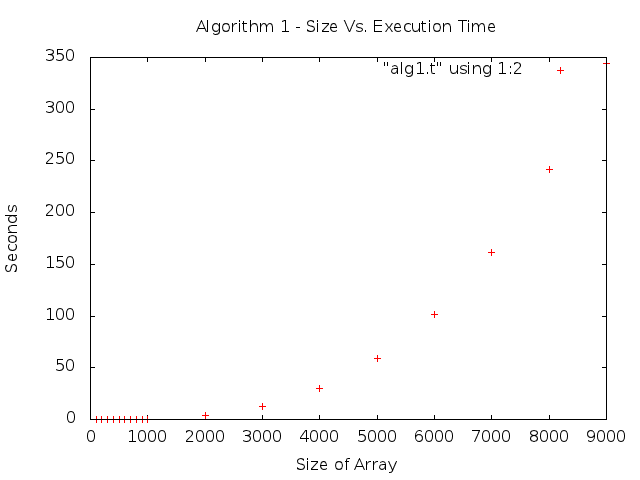
\includegraphics[scale=.5]{timingfiles/alg1plot.png}
			\end{figure}
			\begin{figure}[!htb]
				\centering
				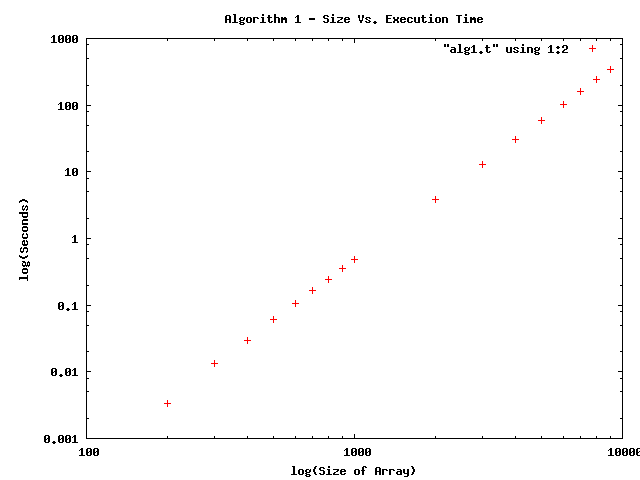
\includegraphics[scale=.5]{timingfiles/alg1plotlog.png}
			\end{figure}
		\newpage
		\subsection{Algorithm 2}
\begin{figure}[!htb]
\centering
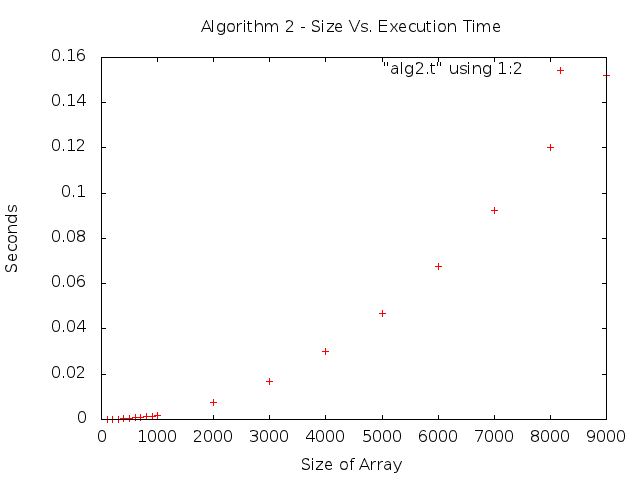
\includegraphics[scale=.5]{timingfiles/alg2plot.png}
\end{figure}
\begin{figure}[!htb]
\centering
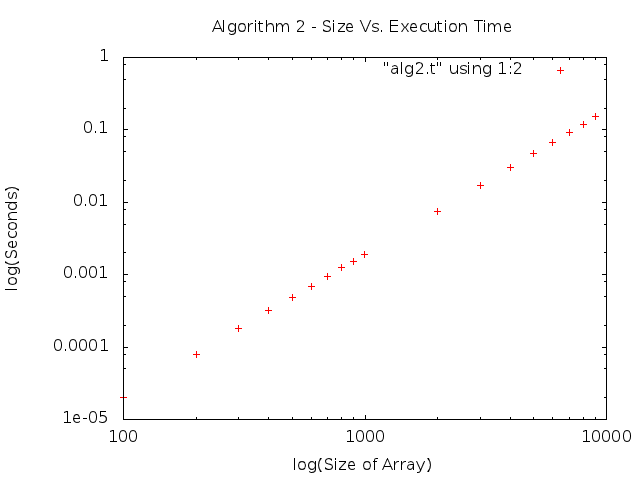
\includegraphics[scale=.5]{timingfiles/alg2plotlog.png}
\end{figure}
		\newpage
		\subsection{Algorithm 3}
\begin{figure}[!htb]
\centering
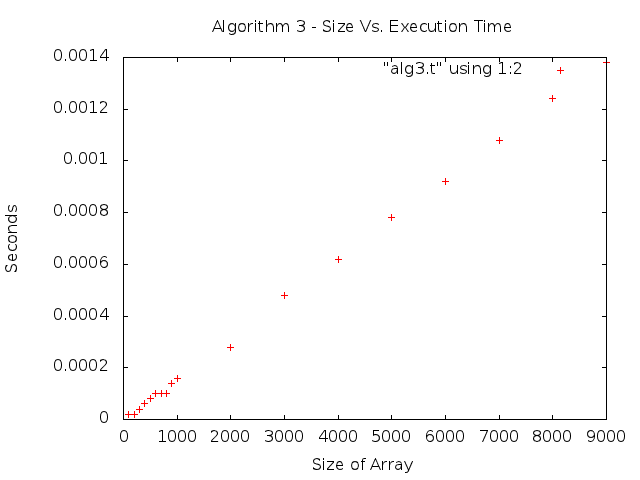
\includegraphics[scale=.5]{timingfiles/alg3plot.png}
\end{figure}
\begin{figure}[!htb]
\centering
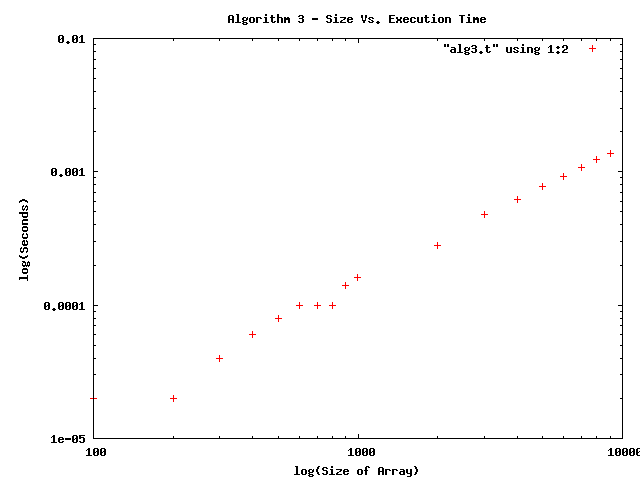
\includegraphics[scale=.5]{timingfiles/alg3plotlog.png}
\end{figure}
\newpage

	\section{Extrapolation and Interpretation}
		\subsection{Extrapolation}
			
		\subsection{Interpretation}

		\subsection{Algorithm 1}
			\subsubsection{Extrapolation}
				$f(n) = 4.71599 \times 10^{-10} \times n^3$\\
				$f(n) = 3600 \to n = 19690$\\
			\subsubsection{Interpretation}
				Slope $= 2.99734$
		
		\subsection{Algorithm 2}
			\subsubsection{Extrapolation}
				$f(n) = 1.87761 \times 10^{-9} \times n^2$\\
				$f(n) = 3600 \to n = 1384678$
			\subsubsection{Interpretation}
				Slope $= 1.99602$
		\subsection{Algorithm 3}
			\subsubsection{Extrapolation}
				$f(n) = 1.74832 \times 10^{-8} \times n \times log(n)$\\
				$f(n) = 3600 \to n = 8984428998 =8.98 \times 10^9$
			\subsubsection{Interpretation}
				Slope $= 1.00506$

	\newpage
	\section{Code}
		\subsection{Files}
			alg1.cpp - function for algorithm 1\\
			alg2.cpp - function for algorithm 1\\
			alg3.cpp - function for algorithm 1\\
			analysis.cpp - code to run algorithm and measure times for the number of array then outputs .t file\\
			makefile - to compile files\\
			maxSubarray.pdf - \\
			maxSubarray.tex - to create pdf filename\\
			test.cpp - allows input of file, and runs algorithm on input file\\
			analysis/ - hold compiled executables for running analysis\\
			test/ - hold compiled executables for running tests on code, and test array files\\
			timingfiles/ - holds files for creating plots\\
			timingfiles/*.t - files that holds rum times for different array sizes\\
			timingfiles/*.gp - code for gnuplot. 2 plots of each algorithm: 1 normal plot, and 1 log-log plot
		\subsection{Algorithm 1}
		\lstinputlisting[language=C++]{alg1.cpp}
		\newpage
		\subsection{Algorithm 2}
		\lstinputlisting[language=C++]{alg2.cpp}
		\newpage
		\subsection{Algorithm 3}
		\lstinputlisting[language=C++]{alg3.cpp}
		

\end{document}
